%%%%%%%%%%%%%%%%%%%%%%%%%%%%%%%%%%%%%%%%%%%%%%%%%%%%%%%%%%%%%%%%%%%%%%%%%%%%%%%%
%2345678901234567890123456789012345678901234567890123456789012345678901234567890
%        1         2         3         4         5         6         7         8
\documentclass[letterpaper, 10 pt, conference]{ieeeconf}  % Comment this line out if you need a4paper
% fix acrobat png issue bug
\pdfminorversion=4
%\documentclass[a4paper, 10pt, conference]{ieeeconf}      % Use this line for a4 paper

\IEEEoverridecommandlockouts                              % This command is only needed if 
                                                          % you want to use the \thanks command

\overrideIEEEmargins                                      % Needed to meet printer requirements.

% See the \addtolength command later in the file to balance the column lengths
% on the last page of the document

% The following packages can be found on http:\\www.ctan.org
%\usepackage{graphics} % for pdf, bitmapped graphics files
%\usepackage{epsfig} % for postscript graphics files
%\usepackage{mathptmx} % assumes new font selection scheme installed
%\usepackage{times} % assumes new font selection scheme installed
%\usepackage{amsmath} % assumes amsmath package installed
%\usepackage{amssymb}  % assumes amsmath package installed

\usepackage{balance}
%\usepackage{subfigure}
%\usepackage[subfigure]{tocloft} 


%\usepackage[colorlinks]{hyperref}
%\usepackage[caption=false]{subfig}


\usepackage{caption}
%\usepackage{subcaption}
\captionsetup{compatibility=false}

\usepackage{benktools}
\usepackage{tikz}
\usetikzlibrary{external}
\usetikzlibrary{positioning,shapes,shadows,arrows, calc, fit, backgrounds, arrows, positioning}
\tikzexternalize[prefix=tikz/]

\usepackage[switch, columnwise]{lineno}
%\linenumbers

\benkhide

\newtheorem{lemma}{Lemma}
\newtheorem{theorem}{Theorem}
\usepackage{amsmath,graphics}
\usepackage{amssymb} 
\usepackage{nicefrac, multirow}
\usepackage{tikz}
\usepackage{bigstrut}
\usepackage{subcaption}

\setlength\bigstrutjot{3pt}
%\usepackage{pgfplots}
%\pgfplotsset{compat=newest}
\usepackage{subfig}
\usepackage{textcomp}
\usetikzlibrary{backgrounds}
\numberwithin{equation}{section} \newtheorem{thm}{Theorem}[section]  
\newtheorem{cor}[thm]{Corollary}    % Corollary environment
\newtheorem{lem}[thm]{Lemma}        % Lemma environment
\newtheorem{dfn}[thm]{Definition}        % Lemma environment
\newtheorem{prop}[thm]{Proposition}  % Proposition environment
\newtheorem{rem}[thm]{Remark}  % Proposition environment
\newtheorem{con}[thm]{Conjecture}  % Proposition environment
\newcommand{\cS}{\mathcal{S}}
\newcommand{\cR}{\mathcal{R}}
\newcommand{\cD}{\mathcal{D}}
\newcommand{\cN}{\mathcal{N}}
\newcommand{\ceq}{\ensuremath{\mathrel{\stackrel{\mathrm{def}}{=}}}} 
\DeclareMathOperator*{\argmin}{arg\,min}
\DeclareMathOperator*{\argmax}{arg\,max}
\newcommand{\rd}{{\mathrm d}}
\newcommand{\p}{\partial}
\tikzstyle{every node}=[font=\small]
%\usepackage{filemod}
\newcommand{\includetikz}[2]{%
\tikzsetnextfilename{#2}%
    \filemodCmp{#1#2.tikz}{#1tikz/#2.pdf}%
        {\tikzset{external/remake next}}{}%
    \input{#1#2.tikz}%
}

\DeclareMathOperator{\J}{J} 
\DeclareMathOperator{\clamp}{clamp} 
\DeclareMathOperator{\interior}{int} 
\DeclareMathOperator{\D}{D} 
\DeclareMathOperator{\Div}{div} 
\DeclareMathOperator{\Sgn}{Sgn} 
\DeclareMathOperator{\Hom}{Hom} 
\DeclareMathOperator{\rank}{rank} 
\DeclareMathOperator{\Vol}{Vol}
\DeclareMathOperator{\Area}{Area}
\DeclareMathOperator{\dVol}{dVol}
\DeclareMathOperator{\supp}{supp} 
\DeclareMathOperator{\Int}{Int} 
\DeclareMathOperator{\Conv}{Conv} 
\DeclareMathOperator{\Cone}{Cone} 
\DeclareMathOperator{\Ker}{Ker} 
\DeclareMathOperator{\Span}{Span} 
\DeclareMathOperator{\Min}{Min} 
\newcommand{\bone}{\mathbf{1}}
\DeclareMathOperator{\tr}{tr} 
\newcommand{\bR}{\mathbb{R}} 
\newcommand{\bZ}{\mathbb{Z}}
\newcommand{\bbeta}{\boldsymbol{\beta}}
\newcommand{\balpha}{\boldsymbol{\alpha}}
\newcommand{\bE}{\mathbb{E}}
\newcommand{\bI}{\mathbb{I}}
\newcommand{\bQ}{\mathbb{Q}}
\newcommand{\bK}{\mathbb{K}}
\newcommand{\bL}{\mathbb{L}} 
\newcommand{\bB}{\mathbb{B}} 
\newcommand{\bbT}{\mathbb{T}} 
\newcommand{\bN}{\mathbb{N}}
\newcommand{\cJ}{\mathcal{J}}
\newcommand{\cI}{\mathcal{I}}
\newcommand{\bS}{\mathbb{S}}
\newcommand{\cL}{\mathcal{L}}
\newcommand{\cF}{\mathcal{F}}
\newcommand{\cH}{\mathcal{H}}
\newcommand{\cU}{\mathcal{U}}
\newcommand{\cK}{\mathcal{K}}
\newcommand{\cB}{\mathcal{B}}
\newcommand{\cV}{\mathcal{V}}
\newcommand{\cZ}{\mathcal{Z}}
\newcommand{\cW}{\mathcal{W}}
\newcommand{\cO}{\mathcal{O}} 
\newcommand{\cC}{\mathcal{C}}
\newcommand{\cT}{\mathcal{T}}
\newcommand{\bbF}{\mathbb{F}}
\newcommand{\cA}{\mathcal{A}}
\newcommand{\cM}{\mathcal{M}}
\newcommand{\cG}{\mathcal{G}}
\newcommand{\cKG}{\mathcal{KG}}
\renewcommand{\phi}{\varphi}
\renewcommand{\div}{\mbox{div}}
\newcommand{\ve}{\varepsilon}
\newcommand{\norm}[1]{\lVert #1 \rVert}
\newcommand{\abs}[1]{\left| #1 \right|}
\newcommand{\ov}[1]{\overline{#1}}
\newcommand{\diff}[4]{\left.\left.\frac{\operatorname{d}}{\operatorname{d}#1}\right.^{#2}#3\right|_{#4}}
\renewcommand{\geq}{\geqslant}
\renewcommand{\leq}{\leqslant}
\renewcommand{\ge}{\geqslant}
\renewcommand{\le}{\leqslant}

\newcommand{\furlp}[1]{\colorbox{blue!10}{\href{run:/home/fulong/academia/library/papers/#1.pdf}{D}}}
\newcommand{\furlb}[1]{\colorbox{blue!10}{\href{run:/home/fulong/academia/library/books/#1.pdf}{D}}}
\newcommand{\fcitep}[1]{\cite{#1}\mbox{\furlp{#1}}}
\newcommand{\fciteb}[1]{\cite{#1}\mbox{\furlb{#1}}}
% we can now use cite as before
% misc defines
\newcommand{\bx}{\mathbf{x}}
\newcommand{\hbx}{\hat{\mathbf{x}}}
\newcommand{\bbx}{\bar{\mathbf{x}}}
\newcommand{\sbx}{\mathbf{x}^{\star}}
\newcommand{\ba}{\mathbf{a}}
\newcommand{\bu}{\mathbf{u}}
\newcommand{\bc}{\mathbf{c}}
\newcommand{\bg}{\mathbf{g}}
\newcommand{\by}{\mathbf{y}}
\newcommand{\bz}{\mathbf{z}}
\newcommand{\bbf}{\mathbf{f}}
\newcommand{\bt}{\mathbf{t}}
\newcommand{\bh}{\mathbf{h}}
\newcommand{\bn}{\mathbf{n}}
\newcommand{\bp}{\mathbf{p}}
\newcommand{\bq}{\mathbf{q}}
\newcommand{\bv}{\mathbf{v}}
\newcommand{\br}{\mathbf{r}}
\newcommand{\bs}{\mathbf{s}}
\newcommand{\bb}{\mathbf{b}}
\newcommand{\bC}{\mathbf{C}}
\newcommand{\bF}{\mathbf{F}}
\newcommand{\bP}{\mathbf{P}}
\newcommand{\bT}{\mathbf{T}}
\newcommand{\bV}{\mathbf{V}}
\newcommand{\hbb}{\hat{\mathbf{b}}}
\newcommand{\hbn}{\hat{\mathbf{n}}}
\newcommand{\bbb}{\bar{\mathbf{b}}}
\newcommand{\hbu}{\hat{\mathbf{u}}}
\newcommand{\bbu}{\bar{\mathbf{u}}}
\newcommand{\bw}{\mathbf{w}}
\newcommand{\mG}{\mathcal{G}}
\newcommand{\mA}{\mathcal{A}}
\newcommand{\mH}{\mathcal{H}}
\newcommand{\mL}{\mathcal{L}}
\newcommand{\mN}{\mathcal{N}}
\newcommand{\mE}{\mathcal{E}}
\newcommand{\mO}{\mathcal{O}}
\newcommand{\mP}{\mathcal{P}}
\newcommand{\mB}{\mathcal{B}}
\newcommand{\mC}{\mathcal{C}}
\newcommand{\mX}{\mathcal{X}}
\newcommand{\mY}{\mathcal{Y}}
\newcommand{\mZ}{\mathcal{Z}}
\newcommand{\mW}{\mathcal{W}}
\newcommand{\mQ}{\mathcal{Q}}
\newcommand{\mR}{\mathcal{R}}
\newcommand{\mU}{\mathcal{U}}
\newcommand{\mD}{\mathcal{D}}
\newcommand{\mF}{\mathcal{F}}
\newcommand{\mS}{\mathcal{S}}
\newcommand{\mK}{\mathcal{K}}
\newcommand{\mV}{\mathcal{V}}
\newcommand{\mI}{\mathcal{I}}
\newcommand{\bG}{\mathbf{G}}
\newcommand{\bA}{\mathbf{A}}
\newcommand{\bW}{\mathbf{W}}
\newcommand{\hmX}{\hat{\mathcal{X}}}
\newcommand{\hmU}{\hat{\mathcal{U}}}
\newcommand{\bmX}{\bar{\mathcal{X}}}
\newcommand{\bmU}{\bar{\mathcal{U}}}
\newcommand{\mT}{\mathcal{T}}
\newcommand{\mM}{\mathcal{M}}
\newcommand{\bPhi}{\boldsymbol{\Phi}}
\newcommand{\bGamma}{\boldsymbol{\Gamma}}
\newcommand{\hbpsi}{\hat{\boldsymbol \psi}}
\newcommand{\bPsi}{\boldsymbol \Psi}
\newcommand{\bpsi}{\boldsymbol{\psi}}
\newcommand{\sS}[1]{\sqrt{\Sigma_{#1}}}
\newcommand{\shS}[1]{\sqrt{\hat{\Sigma}_{#1}}}
\newcommand{\sd}{\texttt{sd}}
\DeclareMathOperator{\Cov}{Cov}
\DeclareMathOperator{\Tr}{tr}
\DeclareMathOperator{\st}{s.t.}
\DeclareMathOperator{\dt}{dt}
\DeclareMathOperator{\Vect}{vec}
\DeclareMathOperator{\diag}{diag}
%\DeclareMathOperator{\argmin}{arg\,min}

\captionsetup{font={footnotesize}}

\newcommand{\specialcell}[2][c]{ \begin{tabular}[#1]{@{}c@{}}#2\end{tabular}}

\newcommand\independent{\protect\mathpalette{\protect\independenT}{\perp}}
\def\independenT#1#2{\mathrel{\rlap{$#1#2$}\mkern2mu{#1#2}}}

\newcommand{\limit}[1] {\underset{#1}{\text{lim }}}
\newcommand{\infimum}[1] {\underset{#1}{\text{inf }}}
\newcommand{\supremum}[1] {\underset{#1}{\text{sup }}}
\newcommand{\maximum}[1] {\underset{#1}{\text{max }}}
\newcommand{\minimum}[1] {\underset{#1}{\text{min }}}
\newcommand{\myargmax}[1] {\underset{#1}{\text{argmax }}}
\newcommand{\myargmin}[1] {\underset{#1}{\text{argmin }}}
\newcommand{\betadist}{\text{Beta}}

\newcommand{\TODO}[1]{\todo{#1}}


\begin{document}
\title{\LARGE \bf Robust Task Wrench Resistance
	\vspace{-2ex}
	\versionline{0}}
\author{Jeffrey Mahler$^1$, Jacky Liang$^1$, Ken Goldberg$^1$
%\vspace{-2ex}
\thanks{{\small $^1$ University of California, Berkeley, USA; {\tt\small \{jmahler, jackyliang, goldberg\}@berkeley.edu}}}% }
}
\maketitle

\begin{abstract}
%\TODO{Adapted from flyer, probably needs to be toned down}
Advances in Big Data and distributed computing, combined with very large datasets of images and human speech, have produced a series of  data-driven results that surpass decades of research in analytic methods and, in some cases, that surpass human ability.
For example, deep neural networks can now learn to play video games, recognize faces, and translate between languages.
This raises the question: can Big Data and computation produce analogous advances in robot grasping and manipulation?
We introduce the Dexterity-Network (Dex-Net) 1.0, a Cloud-based dataset of 3D object models labelled with parallel-jaw grasps and similarity between objects and grasps based on multi-view Convolutional Neural Networks (CNNs) and grasp heightmaps.
We use Dex-Net in Multi-Armed Bandit (MAB) algorithms to quickly find a grasp with high probability of force closure on an object from a set of 250 candidates. 
We extend previous MAB models to predict grasp quality using similiarity to prior objects and grasps in Dex-Net using Continuous Correlated Beta Processes (CCBPs).
Our initial results suggest that using prior objects from Dex-Net can accelerate grasp planning by up to $10\times$.
%\TODO{More concrete results here as I organize them} 
Code, data, and additional information can be found at: \TODO{Url}
\end{abstract}

\section{Introduction}
\seclabel{introduction}

Cloud-based Robotics and Automation systems exchange data and perform computation via networks instead of operating in isolation with limited computation and memory.
Potential advantages to using the Cloud include Big Data: access to updated libraries of images, maps, and object/product data; and Parallel Computation: access to parallel grid computing for statistical analysis, machine learning, and planning~\cite{kehoe2015survey}.
The advantages have recently been used in vision and speech, where datasets with millions of examples such as ImageNet have produced results~\cite{hannun2014deepspeech, krizhevsky2012imagenet} that surpass those obtained from decades of research on analytic methods.
This suggests that large-scale machine learning of grasps for vast numbers of possible object shapes, object poses, and environment configurations~\cite{goldfeder2011data, lenz2015deep, kappler2015leveraging}, could exhibit scaling effects similar to those observed in computer vision and speech recognition.

\begin{figure}[t!]
\centering
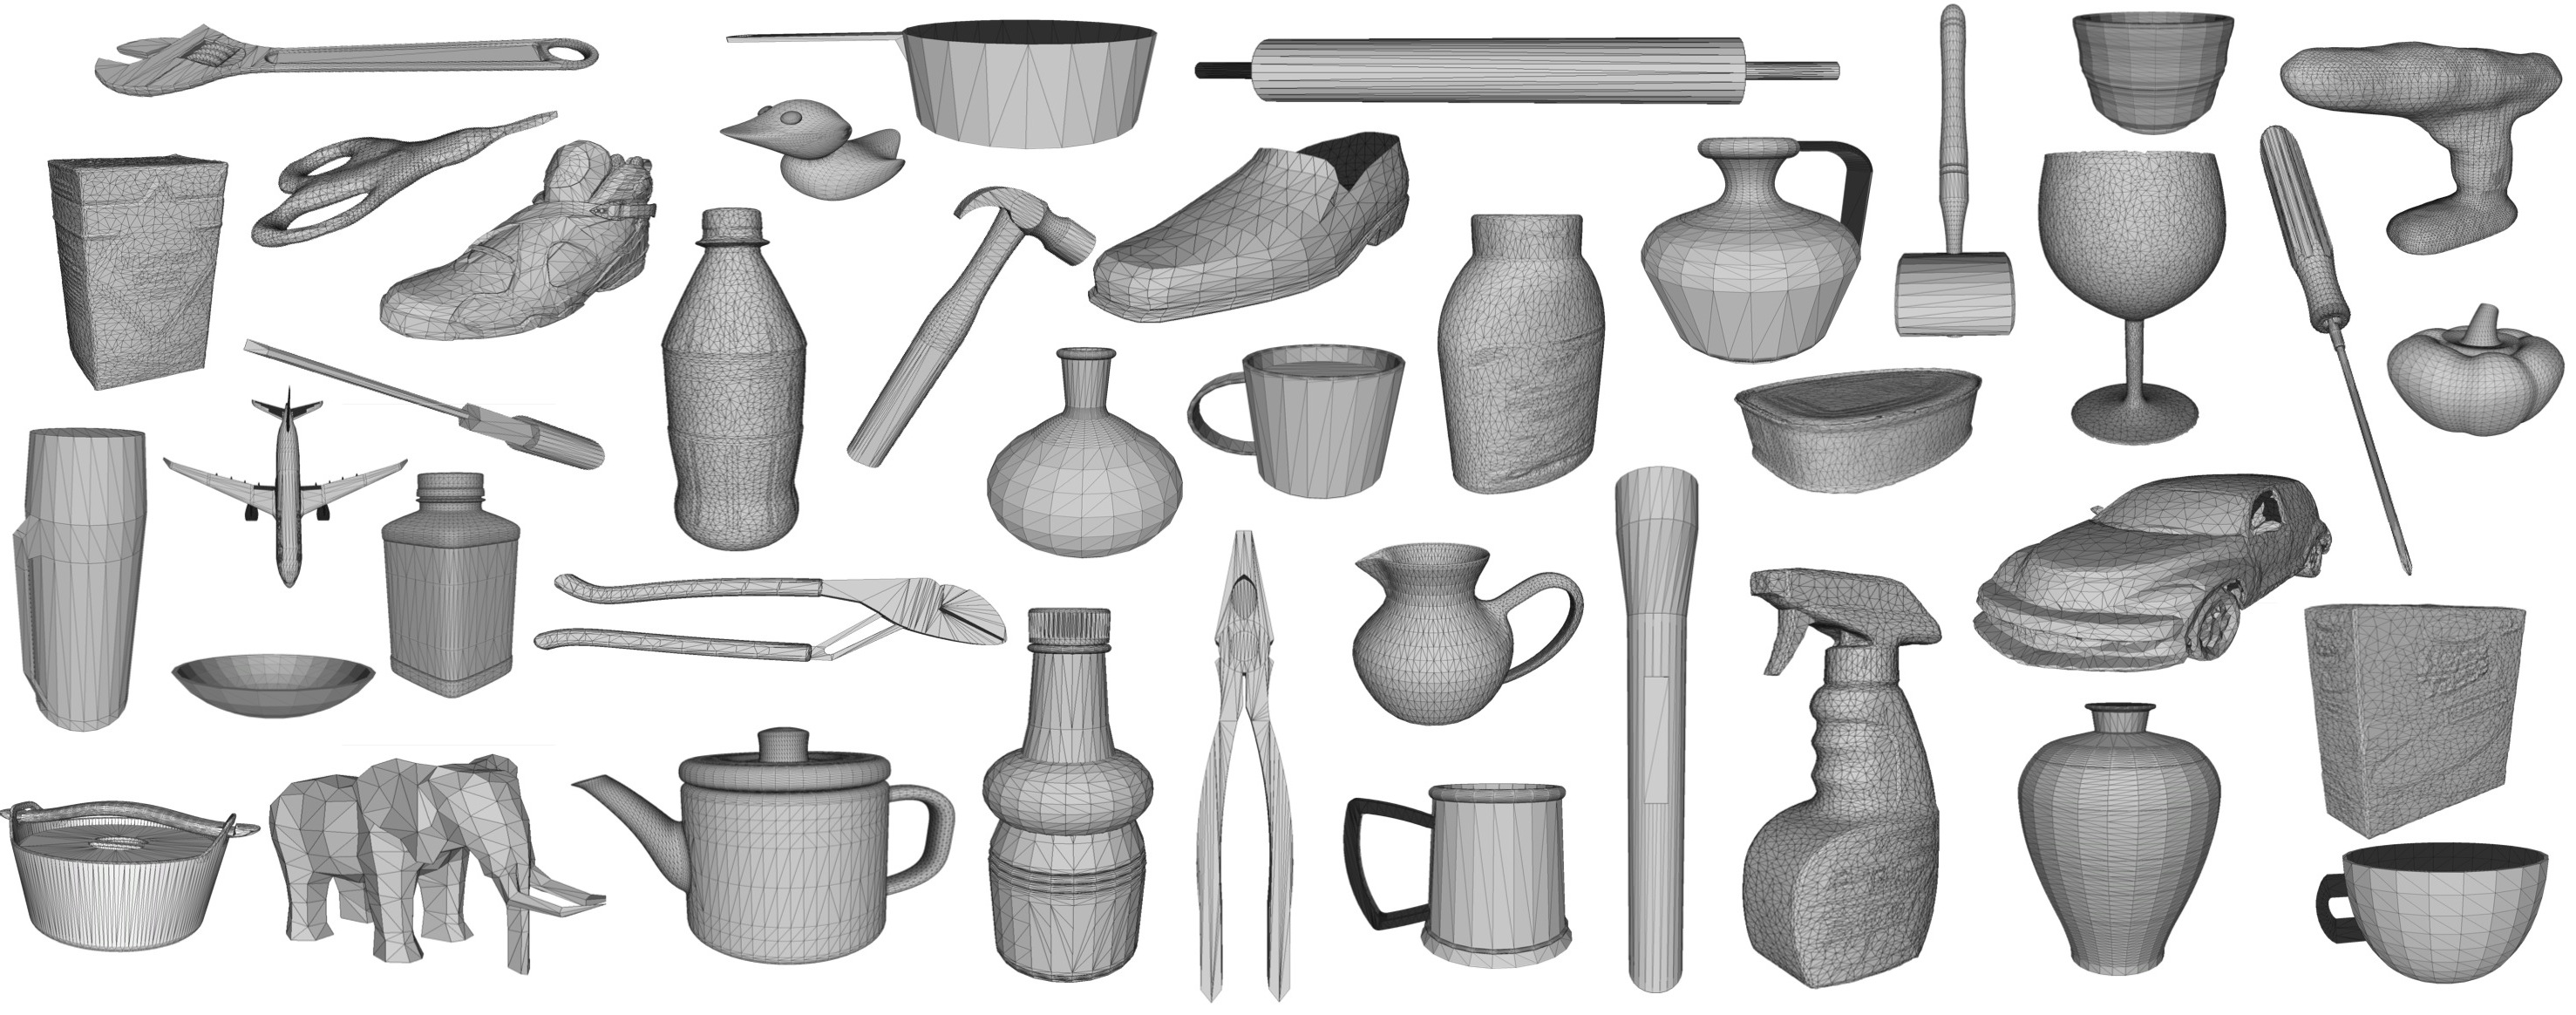
\includegraphics[scale=0.08]{figures/dexnet_collage.jpg}
\caption{Sample of 3D mesh models from the Dex-Net dataset that currently includes over 10,000 models from the KIT object database~\cite{kasper2012kit}, the Yale-CMU-Berkeley object set~\cite{calli2015benchmarking}, 3DNet\cite{wohlkinger20123dnet}, ModelNet~\cite{wu20153d}, and the SHREC 2014 object retrieval challenge dataset~\cite{li2015comparison}. }
\figlabel{dexnet-teaser}
\vspace*{-15pt}
\end{figure}

Our primary contribution is an algorithm based on a Multi-Armed Bandit (MAB) model with correlated rewards to speed up robust planning by learning from a large dataset of prior grasps and 3D object models.
Our algorithm is based on Continuous Correlated Beta Processes (CCBPs)~\cite{goetschalckx2011continuous, montesano2012active}, an efficient model for predicting a belief distribution on the quality of each grasp from prior data.

To study scaling effects we developed Dex-Net 1.0, a growing dataset that currently includes over 10,000 3D object models scaled to fit within a PR2 gripper and selected to reflect objects that could be encountered in warehousing or the home such as containers, tools, tableware, and toys.
~\figref{dexnet-teaser} shows a sample of the objects in the dataset.
%Dex-Net contains laser-scanned 3D mesh models from the KIT object database~\cite{kasper2012kit}, the Amazon Picking Challenge objects, BigBIRD~\cite{singh2014bigbird}, and YCB~\cite{calli2015benchmarking} to reflect physical objects commonly used for benchmarking in grasping research.
%The dataset also includes synthetic 3D mesh models from shape classification datasets such as 3DNet~\cite{wohlkinger20123dnet}, ModelNet~\cite{wu20143d}, and the SHREC 2014 large scale object retrieval challenge~\cite{li2015comparison} to approach larger scales.
Dex-Net also contains approximately 2.5 million parallel-jaw grasps, as each object is labelled with up to 250 grasps and an estimate of the probability of force closure for each under uncertainty in object pose, gripper pose, and friction coefficient.
To the best of our knowledge, this is the largest dataset used for grasping research to-date.
We also incorporate multi-view Convolutional Neural Networks (MV-CNNs)~\cite{su2015multi}, a state-of-the-art method for 3D shape classification, to efficiently retrieve similar 3D objects. 

We implement our algorithm on Google Compute Engine and store Dex-Net 1.0 on Google Cloud Storage, with a system that can run up to 1,500 instances at once.
Experiments on planning parallel-jaw grasps with high probability of force closure with our algorithm suggest that using 10,000 prior object models from Dex-Net can reduce the average number of samples needed to identify a grasp with high quality by $3.5\times$.
\TODO{Update with final results}

 







\section{Related Work}
\seclabel{related}

For a survey of the substantial literature on grasping, see Prattichizzo and Trinkle~\cite{prattichizzo2008grasping}.
Research on grasp planning has focused on finding grasps by maximizing an analytic grasp quality metric based on wrench space (WS), such as the ability to resist external perturbations to the object based on the grasp WS~\cite{ferrari1992, miller2004graspit}, object WS~\cite{liu2015fast, pollard1994parallel}, or task WS~\cite{kruger2011partial, li1988task}.
WS metrics have been used to synthesize grasps for known objects using sampling-based optimization in software tools such as GraspIt!~\cite{miller2004graspit} or OpenGRASP~\cite{leon2010opengrasp}.
However, analytic WS metrics have been criticized~\cite{balasubramanian2012physical, weisz2012pose} for not being robust to variations in grasp acquistion, such as object shape, pose, material properties, and locations of contact~\cite{cheong2011output, diankov2010automated, weisz2012pose, zheng2005} and for not taking into account the dynamics of the the grasp~\cite{prattichizzo2008grasping}.
%This has motivated work on grasp transfer from a knowledge database to new objects, robust versions of analytic quality metrics with respect to uncertainty in the state of the robot and environment, and synthesis from statistical models of grasping learned from physical data or human labels.

The need to recompute WS metrics to select grasps for every new object motivated research on grasp synthesis by transferring grasps from a database of exemplar objects.
Li and Pollard~\cite{li2005shape} generated grasps by matching object shapes to human hand postured in a database.
Goldfelder et al.~\cite{goldfeder2009columbia} developed the Columbia grasp database, a database of 1,814 distinct models and over 200,000 force closure grasps generated using the Eigengrasp planner in GraspIt!~\cite{ciocarlie2009}.
The authors later used synthetic partial depth maps of objects in the database to match robot sensor data to precomputed grasps, using the Iterated Closest Point (ICP) algorithm to align the coordinate frames of the depth maps~\cite{goldfeder2009data, goldfeder2011data}.
Kehoe et al.~\cite{kehoe2013cloud} created a Cloud-based system to transfer grasps evaluated by probability of force closure on objects in a database to a physical robot by indexing the objects with the Google Goggles object recognition engine.
Recent research has also studied grasp transfer from objects of the same category by warping contacts betwen corresponding points on a shape surface and using local rigid alignment and contact interpolation~\cite{hillenbrand2012transferring, stouraitis2015functional} or by interpolating grasps and shapes over a vector space representation called a Grasp Moduli Space~\cite{pokorny2014grasp, pokorny2013grasp}.

Another line of research focused on making analytic grasp metrics robust to imprecision in perception and control~\cite{goldberg1990bayesian, stulp2011learning, zheng2005}.
Brook, Ciocarlie, and Hsiao~\cite{brook2011collaborative, hsiao2011bayesian} developed a Bayesian framework to evaluate both the expected epsilon quality and the probability of physical success on a PR2 given uncertainty in object identity, object pose, and gripper positioning on deterministic mesh and point cloud models. 
Weisz et al.~\cite{weisz2012pose} found that grasps ranked by probability of force closure subject to perturbations of object pose in simulation were empirically more successful on a physical robot than grasps planned using deterministic WS metrics. 
Kim et al.~\cite{kim2012physically} planned grasps using the expected epsilon quality metric~\cite{ferrari1992} under dynamics and uncertainty in pose, and found that the robust metric has a higher correlation with physical grasp success.
Recent research has also studied grasping under object shape uncertainty resulting from imprecision of object segmentations in images~\cite{christopoulos2007handling}, part tolerancing in manufacturing~\cite{kehoe2012estimating, kehoe2012toward, panahi2015orienting}, or missing and noisy data from depth sensors such as the Kinect modeled with Gaussian process implicit surfaces~\cite{dragiev2013uncertainty, mahler2015gp, laskey2015bandits}.
%Many have also studied caging gripper configurations~\cite{rimon1996caging}, which are a waypoint to form closure grasps for two fingers~\cite{vahedi2008caging, rodriguez2012caging} and may be robust to perturbations in object pose and shape~\cite{diankov2008manipulation, Wan2012_ICRA}.

Recent research has also studied synthesizing grasps by ranking grasps according statistical models learned from human annotations or physical execution~\cite{bohg2014data}.
Saxena et al.~\cite{jiang2011efficient, saxena2008robotic} used a logistic regression classified to predict grasp affordances in images from human annotated training data.
Lenz et al~\cite{lenz2015deep} used deep learning to detect bounding boxes for parallel-jaw grasps in color and depth images, which was extended to real time by Redmon and Angelova~\cite{redmon2014real}.
Herzog et al.~\cite{herzog2012template, herzog2014learning} extracted "heightmaps" of local object curvature from human demonstrated grasps, construct a library of heightmap templates, and match new sensor data to templates to select grasps similar to the demonstrations.
Detry et al.~\cite{detry2012generalizing} created a low-dimensional representation of object parts and cluster object parts that are grasped similarly to form a shape library of prototypical grasp parts, and show that this representation can be transferred to real sensor data~\cite{detry2013learning}.
Kappler et al.~\cite{kappler2015leveraging} trained a deep neural network to predict grasp success for a Barett hand measured by human annotations and the results of simulations on a database of synthetic pointclouds of objects.
Deep learning~\cite{krizhevsky2012imagenet} has also ben used in robotics for learning visuomotor policies for specific manipulation tasks~\cite{levine2015end} and recurrent control policies for cutting fruits vegetables from joint angles and end-effector forces~\cite{lenzdeepmpc}.
%Recently, several other works have proposed to form a huge database of grasps on synthetic objects from simulation outcomes~\cite{michalikg3db} or physical execution~\cite{tellex}.
In comparison, we learn a model to predict a Bayesian distribution on the probability of force closure for a grasp on an object based on similarity to a set of prior grasps and objects in a database, and use our model to actively decide the next grasp to evaluate using Multi-Armed Bandits.

Our work is also closely related to research on actively selecting grasps for building a statistical model of grasp quality from fewer examples.
Several works have searched for successful grasps using belief space planning to minimze uncertainty~\cite{hsiao2007grasping, kahnactive, fischinger2015learning}, but without use of an explicit grasp quality metric to guide the search.
Kehoe et al.~\cite{kehoe2012estimating} proposed iterative pruning, an algorithm for evaluating the probability of force closure for a set of candidate grasps while discrading grasps known to have poor quality.
Detry et al.~\cite{detry2011learning} estimated a full continuous density function over grasp poses using kernel density estimation and adaptively acquired samples by pruning unsuccessful grasps.
Kroemer et al.~\cite{kroemer2010combining} developed a reinforcement learning approach to grasp selection based on seeding hypotheses via imitation learning and Gaussian process upper-confidence bounds for active grasp acquisition.
Boularias et al.~\cite{boularias2014efficient, boularias2015learning} used a Gaussian process Bayesian Optimization model for selecting grasps on cluttered piles of rocks.
Salaganicoff et al.~\cite{salganicoff1996active} used active learning to decide the next grasp to execute on a physical robot while learning a predicitve model of empirical success from range sensors.
Similarly, Montesano and Lopes~\cite{montesano2012active} used Continuous Correlated Beta Processes~\cite{goetschalckx2011continuous} to actively acquire grasp executions on a physical robot, measuring correlations from the responses to a bank of image filters designed to detect grasp affordances such as edges.
Recently, Laskey et al.~\cite{laskey2015bandits} showed that Multi-Armed Bandit (MAB) algorithms can be used to accelerate the identification of grasps with high probability of force closure under uncertainty in shape, pose, and friction in 2D.
MAB algorithms trade off gaining information about grasps that have been sampled fewer times with exploiting the grasp with the highest estimated quality given the past samples.
In this work we extend the model of Laskey et al.~\cite{laskey2015bandits} to 3D and to utilize similarity between grasps across objects from Dex-Net with CCBPs to further reduce the number of samples needed to converge to a grasp with high quality.












\section{Acknowledgments}
{\footnotesize
This research was performed in UC Berkeley's Automation Sciences Lab under the UC Berkeley Center for Information Technology in the Interest of Society (CITRIS) ``People and Robots" Initiative: http://robotics.citris-uc.org.
The authors were supported in part by the U.S. National Science Foundation under NRI Award IIS-1227536, by grants from Google, UC Berkeley's Algorithms, Machines, and People Lab; the Knut and Alice Wallenberg Foundation; the NSF-Graduate Research Fellowship; and the Department of Defense (DoD) through the National Defense Science \& Engineering Graduate Fellowship (NDSEG) Program.
We thank our colleagues who gave feedback and suggestions, in particular Pieter Abbeel, Animesh Garg, Kevin Jamieson, Sanjay Krishnan, Sergey Levine, Zoe McCarthy, Stephen McKinley, Sachin Patil, and Nan Tian.
}

%\balance
\bibliographystyle{IEEEtranS}
\bibliography{bibliography}



\end{document}



